\documentclass[20pt, a0paper, portrait,colspace=5pt,blockverticalspace=5pt]{tikzposter}
\title{Tikz Poster Example}
\author{Overleaf Team}
\date{\today}
\usepackage[default]{raleway}
\usepackage{xcolor}
\institute{Overleaf Institute}
%\usetheme{Board}
\usepackage{background}
\backgroundsetup{scale = 1, angle = 0, opacity = 1,
   contents = {
\includegraphics[width = \paperwidth,
   height = \paperheight, keepaspectratio]
   {background.pdf}}}
  
\newcommand{\fr}[1]{}
\newcommand{\en}[1]{#1} 
   
   \definebackgroundstyle{samplebackgroundstyle}{
\draw[inner sep=0pt, line width=0pt, draw opacity =0, fill opacity=0]
(0,0) rectangle (0,0);
}
\usebackgroundstyle{samplebackgroundstyle} 

\definecolor{color1}{HTML}{275562}

\defineblockstyle{titleblock}{
titlewidthscale=0.9, bodywidthscale=1,titleleft,
titleoffsetx=0pt, titleoffsety=0pt, bodyoffsetx=0mm, bodyoffsety=5mm,
bodyverticalshift=10mm, roundedcorners=5, linewidth=2pt,
titleinnersep=6mm, bodyinnersep=1cm
}{
\draw[color=color1, fill=blockbodybgcolor,
rounded corners=\blockroundedcorners] (blockbody.south west)
rectangle (blockbody.north east);
\ifBlockHasTitle
\draw[color=color1, fill=blocktitlebgcolor,
rounded corners=\blockroundedcorners] (blocktitle.south west)
rectangle (blocktitle.north east);
\fi
}


\defineblockstyle{normalblock}{
titlewidthscale=0.9, bodywidthscale=1,titleleft,
titleoffsetx=0pt, titleoffsety=0pt, bodyoffsetx=0mm, bodyoffsety=15mm,
bodyverticalshift=10mm, roundedcorners=5, linewidth=2pt,
titleinnersep=6mm, bodyinnersep=1cm
}{
\draw[color=color1, fill=blockbodybgcolor,
rounded corners=\blockroundedcorners] (blockbody.south west)
rectangle (blockbody.north east);
\ifBlockHasTitle
\draw[color=color1, fill=blocktitlebgcolor,
rounded corners=\blockroundedcorners] (blocktitle.south west)
rectangle (blocktitle.north east);
\fi
}


\defineblockstyle{instituteblock}{
titlewidthscale=0.9, bodywidthscale=1,titleleft,
titleoffsetx=0pt, titleoffsety=0pt, bodyoffsetx=0mm, bodyoffsety=0mm,
bodyverticalshift=0mm, linewidth=0pt,
titleinnersep=0mm, bodyinnersep=0cm
}{
\draw[draw=none,color=blocktitlebgcolor,fill=blockbodybgcolor] (blockbody.south west)
rectangle (blockbody.north east);
\ifBlockHasTitle
\draw[draw=none,color=blocktitlebgcolor, fill=blocktitlebgcolor] (blocktitle.south west)
rectangle (blocktitle.north east);
\fi
}


\tikzposterlatexaffectionproofoff
\usepackage{tikz}
\usetikzlibrary{positioning}% To get more advances positioning options
\usetikzlibrary{arrows}% To get more arrow heads

\title{A tempered Sequential Monte Carlo Method for estimating the number of
variants in metagenomic samples}
\author{Anne-Laure Abraham¹, {\bf Daniel Bonnéry¹$^,$²}, Nicolas Chopin³, Guillaume Kon Kam King¹, Sebastien Leclercq¹, Ouleye Sidibe¹}

\settitle{ \phantom{.}
\\[\TP@titlegraphictotitledistance]
{\color{color1}\Huge\bf\color{titlefgcolor} { \Huge \@title \par}}
\vspace*{1em}
{\color{color1}\large \@author \par} \vspace*{1em} 
}


\usepackage{caption}
\usepackage{subcaption}
\usepackage{pifont}
    \usetikzlibrary{positioning}
    \usetikzlibrary{backgrounds}
    \usetikzlibrary{arrows.meta}
\usetikzlibrary{3d, calc}



\newcommand\indexsum[1]{\mathbf{\bar{#1}}}
\newcommand\indexvec[1]{\mathbf{#1}}
\usepackage{graphicx}
\usepackage{subcaption}
\usepackage[textwidth=8em,textsize=small]{todonotes}
\usepackage{amsmath}
\usepackage{amssymb}
\usepackage{amsfonts}
\usepackage{float}
\usepackage{natbib}
\usepackage{blkarray}\usepackage{bbold}
\usepackage{ulem} %To strike out things using \sout
\usepackage{econometrics} % for bold greek letters, e.g. \valpha instead of \alpha
\usepackage{enumerate}
\usepackage{xcolor}  % Coloured text etc.
% 
\usepackage{multirow}
\usepackage{todonotes}
\newcommand{\afaire}[1]{\todo[linecolor=red,backgroundcolor=red!25,bordercolor=red]{#1}}
\usepackage{stmaryrd}
\usepackage{algorithm}
\usepackage{algorithmicx}
\usepackage{algpseudocode}

\usepackage{collcell}
\usepackage{colortbl,dcolumn}

\usepackage{dsfont}


    \usetikzlibrary{positioning}
    \usetikzlibrary{backgrounds}
\usetikzlibrary{arrows, automata}
    \usetikzlibrary{arrows.meta}
\usetikzlibrary{fit}
    \usepackage{caption}
\newcommand{\code}[1]{\colorbox{light-gray}{\texttt{#1}}}

\newcommand\thevector[4]{{#1}^{{#2}^{{#3}^{{#4}}}}}

\newcommand\A{\thevector{\mathbf{1}}{0}{0}{0}}
\newcommand\C{\thevector{0}{\mathbf{1}}{0}{0}}
\newcommand\G{\thevector{0}{0}{\mathbf{1}}{0}}
\newcommand\T{\thevector{0}{0}{0}{\mathbf{1}}}

\begin{document}

%\maketitle[titletotopverticalspace=12cm]
\makeatletter
    \setlength{\TP@blocktop}{.48\textheight}
\makeatother

%\begin{columns}
%    \column{0.2}
%\useblockstyle{instituteblock} 
%\block{}{\color{color1}\normalsize\underline{Équipe de recherche}\\
%¹ Université Paris-Saclay, INRAE, MaIAGE, Jouy-en-Josas, France\\
%² Ensae, Palaiseau, France\\
%³ Crest,
%⁴ Ensae}
%    \column{0.8}
\begin{columns}
\column{0.15}
\column{0.65}
\useblockstyle{titleblock} 
\block{}
{\color{color1}
    {\Huge \bf A tempered Sequential Monte Carlo Method for estimating the number of
variants in metagenomic samples}\\

\Large
Anne-Laure Abraham$^{1}$, {\bf Daniel Bonnéry$^{1,4}$}, Nicolas Chopin$^{3}$, Guillaume Kon Kam King$^{1,4}$, Sebastien Leclercq$^{2}$, Ouleye Sidibe$^{2}$. \hspace*{1cm}\normalsize $^1$ Inrae, MaIAGE, $^2$ Inrae, $^3$ Ensae-Crest,$^4$ Ensae
}
\column{0.2}
\end{columns}
%\end{columns}




\useblockstyle{normalblock} 
\begin{columns}
    \column{0.33}
   
    \block{1. Parameters}{
The variants ($\tau$), the proportions in each sample ($\pi$), the mearsurement error rate ($\epsilon$)

$$\tau=\begin{blockarray}{ccccc}
    {\scriptstyle g=1}&{\scriptstyle g=2}&\cdots&{\scriptstyle g=G}&\\
    \begin{block}{(cccc)c}
 G&G&\cdots&G&{\scriptstyle v=1}\\   
 C&T&\cdots&T&{\scriptstyle v=2}\\   
 \vdots&\vdots&\ddots&\vdots&{\scriptstyle \vdots}\\   
 T&A&\cdots&T&{\scriptstyle v=V}\\
    \end{block}
\end{blockarray} =    \begin{blockarray}{ccccc}
    {\scriptstyle g=1}&{\scriptstyle g=2}&{\scriptstyle \cdots}&{\scriptstyle g=G}&\\
    \begin{block}{(cccc)c}
 \G&\G&\cdots&\G&{\scriptstyle v=1}\\   
 \C&\T&\cdots&\T&{\scriptstyle v=2}\\   
 \vdots&\vdots&\ddots&\vdots&{\scriptstyle \vdots}\\   
 \T&\A&\cdots&\T&{\scriptstyle v=V}\\
    \end{block}
\end{blockarray} $$ 

$$\pi=\begin{blockarray}{cccc}
    {\scriptstyle s=1}&{\scriptstyle \cdots}&{\scriptstyle s=S}&\\
    \begin{block}{(ccc)c}
    1&0.25&0.1&{\scriptstyle g=1}\\
    0&0.25&0.5&{\scriptstyle \vdots}\\
    0&0.25&0.2&{\scriptstyle \vdots}\\
    0&0.25&0.1&{\scriptstyle \vdots}\\
    0&0&0.1&{\scriptstyle g=G}\\
    \end{block}
\end{blockarray},~~~ \epsilon=\begin{pmatrix}
\epsilon_{1,1}&\cdots&\epsilon_{1,4}\\
\vdots&&\vdots\\
\epsilon_{4,1}&\cdots&\epsilon_{4,4}\\
    \end{pmatrix}$$

}
    \column{0.33}
 \block{2. Observations}{

\en{A 3-dimensional array of counts of nucleotides.}
\fr{On observe un tableau tridimensionel de comptages}
$$\left(n_{v,s,a}\right)_{\footnotesize\begin{array}{cl}
v\in\{1,\ldots,V\}&\text{(position)}\\
s\in\{1,\ldots,S\}&\text{(sample)}\\
a\in \{A,C,G,T\}&\text{(nucleotide)}\end{array}}$$
}
    \block{3. Likelihood}{
\begin{eqnarray*}\lefteqn{\mathcal{L}\left(n | \pi, \tau,\epsilon,n_{\indexvec{v},\indexvec{s},\indexsum{a}} \right)}\nonumber\\& =& \prod_{v=1}^{V} \prod_{s = 1}^{S} (n_{v,s,\indexsum{a}})!\times\frac{\prod_{a = 1}^{4} \left( \sum_{g = 1}^{G}\sum_{b=1}^{4} \tau_{v,g,b}\epsilon_{b,a} \pi_{g,s}  \right)^{n_{v,s,a}}}{\prod_{a = 1}^{4}n_{v,s,a}!}\nonumber\\
& =&\prod_{v=1}^{V} \prod_{s = 1}^{S} (n_{v,s,\indexsum{a}})!\times\frac{\prod_{a = 1}^{4} \left( \sum_{g = 1}^{G} \rho_{v,g,a} \pi_{g,s}  \right)^{n_{v,s,a}}}{\prod_{a = 1}^{4}n_{v,s,a}!},\end{eqnarray*}
with $\rho_{v,g,a}=\sum_{b\in\llbracket 1,4\rrbracket}\tau_{v,g,b}\epsilon_{b,a}.$
}
    \column{0.33}
\block{4. Priors}{}   
 

\block{5. Desman}{} 
 
\end{columns}
\begin{columns}
    \column{0.66}
    \block{Mixture model}{
 
 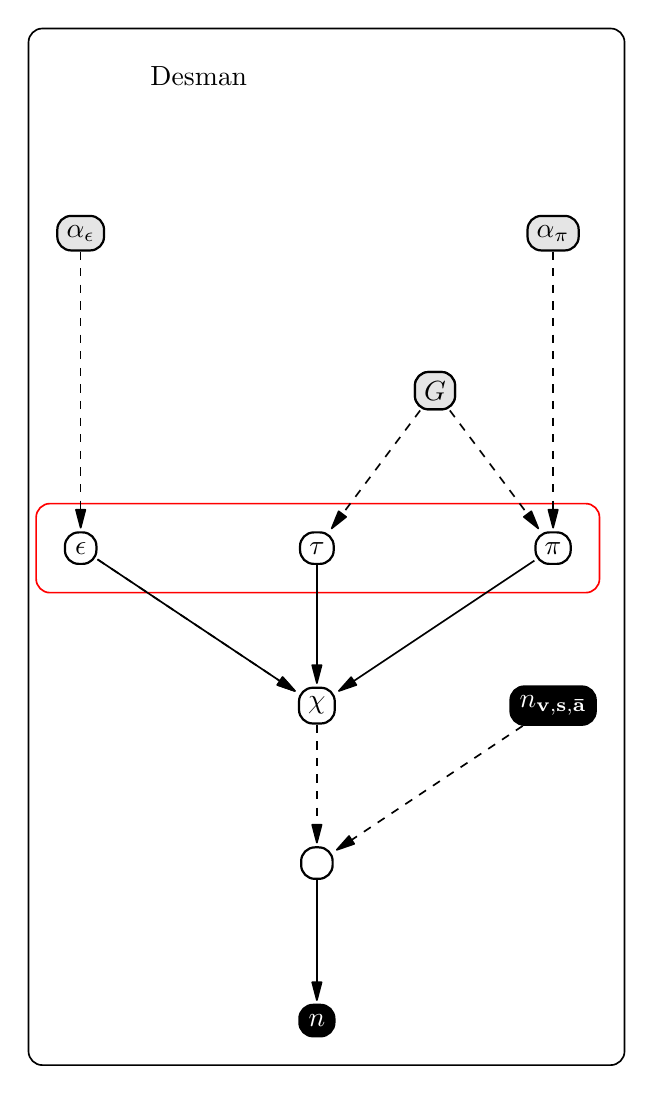
\begin{tikzpicture}[y=-2cm,x=3cm,
            > = {Stealth[inset=0pt,length=8pt,angle'=28,round]}, % arrow head style
            shorten > = 1pt, % don't touch arrow head to node
            auto,
%            node distance =1cm and 3cm, % distance between nodes
            semithick, % line style
            box/.style = {draw,red,inner sep=10pt,rounded corners=5pt}
        ]

        \tikzstyle{every state}=[
        rectangle,
        rounded corners=5pt,
            draw = black,
            thick,
            fill = white,
            minimum size = 4mm
        ]

 		\node at (1.5,1) (tt) {Desman};
        \node at (1.5,1) (blank) {};
        \node[state,fill=black!10] at (2.5,3) (G) {$G$};
        \node[state,fill=black!10] at (3,2) (alphapi) {$\alpha_\pi$};
        \node[state,fill=black!10] at (1,2) (alphaepsilon) {$\alpha_{\epsilon}$};
        \node[state] (tau) at (2,4) {$\tau$};
        \node[state] (epsilon) at (1,4) {$\epsilon$};
        \node[state] (pi) at (3,4) {$\pi$};
        \node[state] (chi) at (2,5) {$\chi$};
        %%\node (theta) at (0.5,4) {$\Theta$};
        \node[state,text=white,fill=black] (n) at (2,7) {$n$};
        \node[state,text=white,fill=black] (nvs) at (3,5)  {$n_{\indexvec{v},\indexvec{s},\indexsum{a}}$};
        \node[state] (m) at (2,6) {$\countdetail$};

         \node[box,fit=(tau) (pi) (epsilon)] {};
         
        \path[->,dashed] (alphapi) edge node {} (pi);
        \path[->,dashed] (alphaepsilon) edge node {} (epsilon);
        \path[->] (epsilon) edge node {} (chi);
        \path[->] (tau) edge node {} (chi);
        \path[->] (pi) edge node {} (chi);
        \path[->,dashed] (chi) edge node {} (m);
        \path[->,dashed] (epsilon) edge node {} (chi);
        \path[->,dashed] (nvs) edge node {} (m);
        \path[->,dashed] (G) edge node {} (tau);
        \path[->,dashed] (G) edge node {} (pi);
        \node[state,fill=black!10] at (2.5,3) (G) {$G$};
        \path[->] (m) edge node {} (n);
       
       
         \node[box,color=black,fit= (tt) (tau) (pi) (epsilon) (alphaepsilon) (m) (nvs) (n) (chi) (alphapi)] {};
        
    \end{tikzpicture}%
 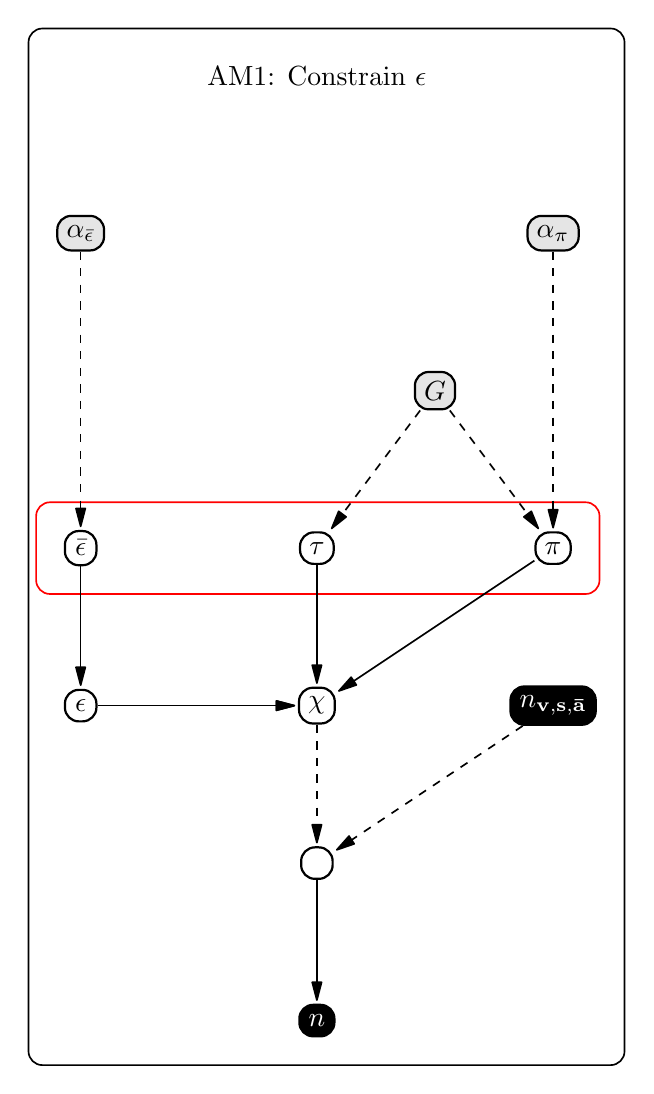
\begin{tikzpicture}[y=-2cm,x=3cm,
            > = {Stealth[inset=0pt,length=8pt,angle'=28,round]}, % arrow head style
            shorten > = 1pt, % don't touch arrow head to node
            auto,
%            node distance =1cm and 3cm, % distance between nodes
            semithick, % line style
            box/.style = {draw,red,inner sep=10pt,rounded corners=5pt}
        ]

        \tikzstyle{every state}=[
        rectangle,
        rounded corners=5pt,
            draw = black,
            thick,
            fill = white,
            minimum size = 4mm
        ]

        \node at (2,1) (tt) {AM1: Constrain $\epsilon$};
        \node at (1.5,1) (blank) {};

        \node[state,fill=black!10] at (2.5,3) (G) {$G$};
        \node[state,fill=black!10] at (3,2) (alphapi) {$\alpha_\pi$};
        \node[state,fill=black!10] at (1,2) (alphaepsilon) {$\alpha_{\bar\epsilon}$};
        \node[state] at (1,4) (barepsilon) {${\bar\epsilon}$};
        \node[state] (tau) at (2,4) {$\tau$};
        \node[state] (epsilon) at (1,5) {$\epsilon$};
        \node[state] (pi) at (3,4) {$\pi$};
        \node[state] (chi) at (2,5) {$\chi$};
        %%\node (theta) at (0.5,4) {$\Theta$};
        \node[state,text=white,fill=black] (n) at (2,7) {$n$};
        \node[state,text=white,fill=black] (nvs) at (3,5)  {$n_{\indexvec{v},\indexvec{s},\indexsum{a}}$};
        \node[state] (m) at (2,6) {$\countdetail$};

         \node[box,fit= (tau) (pi) (barepsilon)] {};
         
        \path[->,dashed] (alphapi) edge node {} (pi);
        \path[->,dashed] (alphaepsilon) edge node {} (barepsilon);
        \path[->] (barepsilon) edge node {} (epsilon);
        \path[->] (epsilon) edge node {} (chi);
        \path[->] (tau) edge node {} (chi);
        \path[->] (pi) edge node {} (chi);
        \path[->,dashed] (chi) edge node {} (m);
        \path[->] (epsilon) edge node {} (chi);
        \path[->,dashed] (nvs) edge node {} (m);
        \path[->] (m) edge node {} (n);
        \path[->,dashed] (G) edge node {} (tau);
        \path[->,dashed] (G) edge node {} (pi);
       
       
         \node[box,color=black,fit= (tt) (tau) (pi) (barepsilon) (alphaepsilon) (m) (nvs) (n) (chi) (alphapi)] {};
        
    \end{tikzpicture}%
 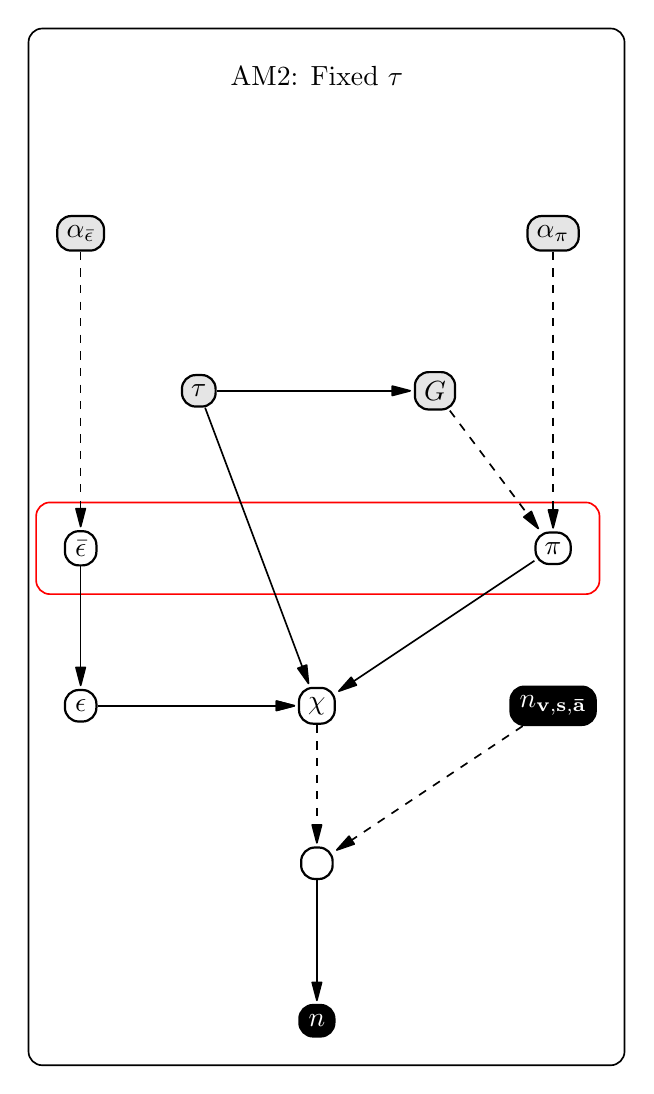
\begin{tikzpicture}[y=-2cm,x=3cm,
            > = {Stealth[inset=0pt,length=8pt,angle'=28,round]}, % arrow head style
            shorten > = 1pt, % don't touch arrow head to node
            auto,
%            node distance =1cm and 3cm, % distance between nodes
            semithick, % line style
            box/.style = {draw,red,inner sep=10pt,rounded corners=5pt}
        ]

        \tikzstyle{every state}=[
        rectangle,
        rounded corners=5pt,
            draw = black,
            thick,
            fill = white,
            minimum size = 4mm
        ]

        \node at (2,1) (tt) {AM2: Fixed $\tau$ };

        \node[state,fill=black!10] at (2.5,3) (G) {$G$};
        \node[state,fill=black!10] at (3,2) (alphapi) {$\alpha_\pi$};
        \node[state,fill=black!10] at (1,2) (alphaepsilon) {$\alpha_{\bar\epsilon}$};
        \node[state] at (1,4) (barepsilon) {${\bar\epsilon}$};
        \node[state,fill=black!10] (tau) at (1.5,3) {$\tau$};
        \node[state] (epsilon) at (1,5) {$\epsilon$};
        \node[state] (pi) at (3,4) {$\pi$};
        \node[state] (chi) at (2,5) {$\chi$};
        %\node (theta) at (0.5,4) {$\Theta$};
        \node[state,text=white,fill=black] (n) at (2,7) {$n$};
        \node[state,text=white,fill=black] (nvs) at (3,5)  {$n_{\indexvec{v},\indexvec{s},\indexsum{a}}$};
        \node[state] (m) at (2,6) {$\countdetail$};

         \node[box,fit=  (pi) (barepsilon)] {};
        \path[->,dashed] (alphapi) edge node {} (pi);
        \path[->,dashed] (alphaepsilon) edge node {} (barepsilon);
        \path[->] (barepsilon) edge node {} (epsilon);
        \path[->] (epsilon) edge node {} (chi);
        \path[->] (tau) edge node {} (chi);
        \path[->] (pi) edge node {} (chi);
        \path[->,dashed] (chi) edge node {} (m);
        \path[->] (epsilon) edge node {} (chi);
        \path[->,dashed] (nvs) edge node {} (m);
        \path[->] (m) edge node {} (n);
        \path[->] (tau) edge node {} (G);
        \path[->,dashed] (G) edge node {} (pi);
       
        
       
         \node[box,color=black,fit= (tt) (tau) (pi) (alphaepsilon) (alphapi) (m) (nvs) (n) (chi)] {};
    \end{tikzpicture}%
  \begin{tikzpicture}[y=-2cm,x=3cm,
            > = {Stealth[inset=0pt,length=8pt,angle'=28,round]}, % arrow head style
            shorten > = 1pt, % don't touch arrow head to node
            auto,
%            node distance =1cm and 3cm, % distance between nodes
            semithick, % line style
            box/.style = {draw,red,inner sep=10pt,rounded corners=5pt}
        ]

        \tikzstyle{every state}=[
        rectangle,
        rounded corners=5pt,
            draw = black,
            thick,
            fill = white,
            minimum size = 4mm
        ]


        \node at (2,0) (tt) {AM3: Relax $\rho$ };
        \node[state,fill=black!10] at (2.5,1.5) (G) {$G$};
        \node[state,fill=black!10] at (3,1) (alphapi) {$\alpha_\pi$};
        \node[state,fill=black!10] at (1.5,1) (alpharho) {$\alpha_\rho$};
        \node[state] (pi) at (3,3) {$\pi$};
        \node[state] (chi) at (1.75,4) {$\chi_{\indexvec{v},\indexvec{s},\indexvec{a},\indexsum{b},\indexvec{g}}$};
        \node[state] (rho) at (1.5,3) {$\tilde\rho$};
        \node[state] (tau) at (.5,4) {$\tau$};
        \node[state,text=white,fill=black] (n) at (2,6) {$n$};
        \node[state] (m) at (2,5) {$\countdetail_{\indexvec{v},\indexvec{s},\indexvec{a},\indexsum{b},\indexvec{g}}$};

        \node[state,text=white,fill=black] (nvs) at (3,4) {$n_{\indexvec{v},\indexvec{s},\indexsum{a}}$};
        
        \node[box,fit=(pi) (rho) ] {};
        \path[->,dashed] (alpharho) edge node {} (rho);
        \path[->,dashed] (alphapi) edge node {} (pi);
        \path[->] (pi) edge node {} (chi);
        \path[->] (rho) edge node {} (chi);
        \path[->,dashed] (chi) edge node {} (m);
        \path[->] (rho) edge node {} (tau);
        \path[->,dashed] (nvs) edge node {} (m);
        \path[->] (m) edge node {} (n);
        \path[->,dashed] (G) edge node {} (pi);
        \path[->,dashed] (G) edge node {} (rho);
        
        \node[box,color=black,fit= (tt) (tau) (pi) (alpharho) (alphaepsilon) (m) (nvs) (n) (chi)] {};
    \end{tikzpicture}%
 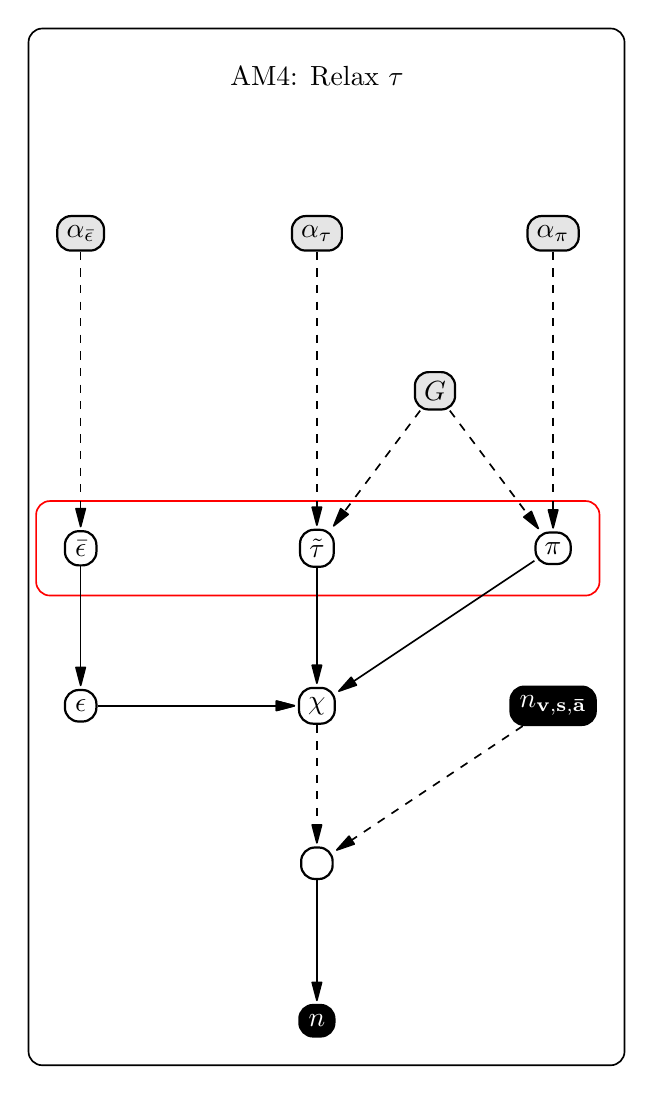
\begin{tikzpicture}[y=-2cm,x=3cm,
            > = {Stealth[inset=0pt,length=8pt,angle'=28,round]}, % arrow head style
            shorten > = 1pt, % don't touch arrow head to node
            auto,
%            node distance =1cm and 3cm, % distance between nodes
            semithick, % line style
            box/.style = {draw,red,inner sep=10pt,rounded corners=5pt}
        ]

        \tikzstyle{every state}=[
        rectangle,
        rounded corners=5pt,
            draw = black,
            thick,
            fill = white,
            minimum size = 4mm
        ]

        \node at (2,1) (tt) {AM4: Relax $\tau$ };
        \node at (1.5,1) (blank) {};

        \node[state,fill=black!10] at (2.5,3) (G) {$G$};
        \node[state,fill=black!10] at (2,2) (alphatau) {$\alpha_\tau$};
        \node[state,fill=black!10] at (3,2) (alphapi) {$\alpha_\pi$};
        \node[state,fill=black!10] at (1,2) (alphaepsilon) {$\alpha_{\bar\epsilon}$};
        \node[state] at (1,4) (barepsilon) {${\bar\epsilon}$};
        \node[state] (tau) at (2,4) {$\tilde\tau$};
        \node[state] (epsilon) at (1,5) {$\epsilon$};
        \node[state] (pi) at (3,4) {$\pi$};
        \node[state] (chi) at (2,5) {$\chi$};
        %\node (theta) at (0.5,4) {$\Theta$};
        \node[state,text=white,fill=black] (n) at (2,7) {$n$};
        \node[state,text=white,fill=black] (nvs) at (3,5)  {$n_{\indexvec{v},\indexvec{s},\indexsum{a}}$};
        \node[state] (m) at (2,6) {$\countdetail$};

         \node[box,fit= (tau) (pi) (barepsilon)] {};
        \path[->,dashed] (alphatau) edge node {} (tau);
        \path[->,dashed] (alphapi) edge node {} (pi);
        \path[->,dashed] (alphaepsilon) edge node {} (barepsilon);
        \path[->] (barepsilon) edge node {} (epsilon);
        \path[->] (epsilon) edge node {} (chi);
        \path[->] (tau) edge node {} (chi);
        \path[->] (pi) edge node {} (chi);
        \path[->,dashed] (chi) edge node {} (m);
        \path[->] (epsilon) edge node {} (chi);
        \path[->,dashed] (nvs) edge node {} (m);
        \path[->] (m) edge node {} (n);
        \path[->,dashed] (G) edge node {} (tau);
        \path[->,dashed] (G) edge node {} (pi);
       
         \node[box,color=black,fit= (tt) (tau) (pi) (barepsilon) (alphaepsilon) (m) (nvs) (n) (chi)] {};
        
    \end{tikzpicture}%
 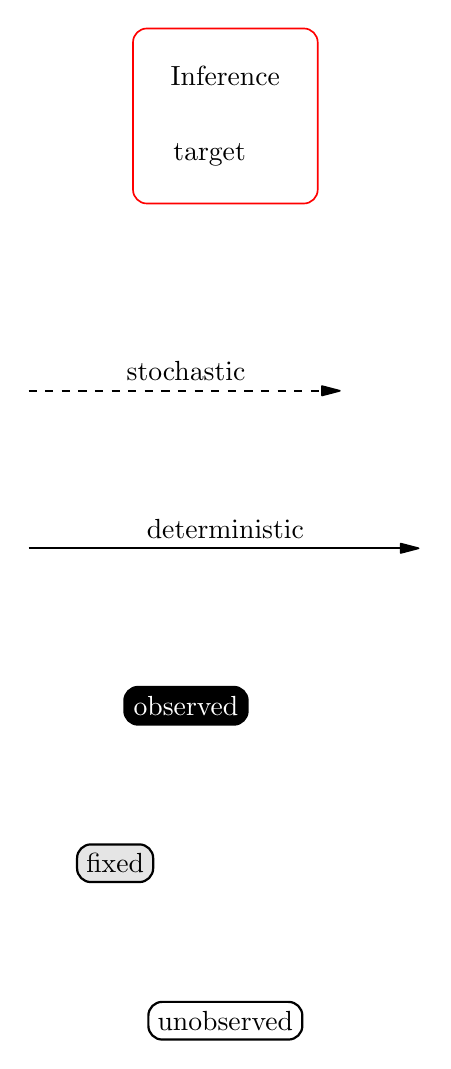
\begin{tikzpicture}[y=2cm,
            > = {Stealth[inset=0pt,length=8pt,angle'=28,round]}, % arrow head style
            shorten > = 1pt, % don't touch arrow head to node
            auto,
%            node distance =1cm and 3cm, % distance between nodes
            semithick, % line style
            box/.style = {draw,red,inner sep=10pt,rounded corners=5pt}
        ]

        \tikzstyle{every state}=[
        rectangle,
        rounded corners=5pt,
            draw = black,
            thick,
            fill = white,
            minimum size = 4mm
        ]

        \node[state,fill=black!10] at (1.1,1) (fixed) {fixed};
        \node[state] at (2.5,0)  (unobserved)  {unobserved};
        \node[state,text=white,fill=black ] at (2,2) (observed)  {observed};
        \path[->] (0,3) edge node {deterministic} (5,3);
        \path[->,dashed] (0,4) edge node {stochastic} (4,4);

        \node at (2.3,5.5) (theta1) {target};
        \node at (2.5,6) (theta2) {Inference};
        \node[box,fit=(theta1) (theta2)] {};
         \end{tikzpicture}
}
    \block{Mixture model}{
$G$ variants, present in different proportions in each sample

$\tau$}
    
    \column{0.33}
    \block{}{}
    \column{0.33}
    \block{References}{
\small{
Dau, H. D., \& Chopin, N. (2022). Waste-free sequential monte carlo. Journal of the Royal Statistical Society Series B: Statistical Methodology, 84(1), 114-148.

Quince, C., Delmont, T. O., Raguideau, S., Alneberg, J., Darling, A. E., Collins, G., \& Eren, A. M. (2017). DESMAN: a new tool for de novo extraction of strains from metagenomes. Genome biology, 18, 1-22.
}}
\end{columns}


\end{document}